\def\CTeXPreproc{Created by ctex v0.2.9, don't edit!}
%\documentclass{beamer}
\documentclass[%handout,
xcolor=pdftex]{beamer}
\mode<presentation> {
  \usetheme{Warsaw}
  \setbeamercovered{transparent}
}
\let\Tiny=\tiny
\usetheme{Singapore}
\usecolortheme{dolphin}
\usepackage{amsmath}
\usepackage{textcomp}
\usepackage{amssymb}
\usepackage{amsthm}
\usepackage{graphicx}
\usepackage{color}
\usepackage{lipsum}
\usepackage{hyperref}
\usepackage{multirow}
\usepackage{bm}
\DeclareMathSymbol{\Phi}{\mathalpha}{operators}{8}
%\setbeamertemplate{headline}{}
\setbeamertemplate{footline}[page number]
\newcommand\Fontvi{\fontsize{9pt}{8}\selectfont}
\newcommand\Fontvii{\fontsize{7pt}{8}\selectfont}
\newcommand{\backupbegin}{
   \newcounter{finalframe}
   \setcounter{finalframe}{\value{framenumber}}
}
\newcommand{\backupend}{
   \setcounter{framenumber}{\value{finalframe}}
}\newtheorem{proposition}{Proposition}
\title{Unit 21: Nonparametric Spectral Density Estimation}
\author[STAT 5170: Applied Time Series, Unit 21]{Taylor R. Brown}
\institute{Department of Statistics, University of Virginia}
\date{Fall 2020}

\AtBeginSubsection[] {
  \begin{frame}<beamer>{Outline}
    \tableofcontents[currentsection,currentsubsection]
  \end{frame}
}



\begin{document}


\frame{\titlepage}


\begin{frame}
\frametitle{Readings for Unit 21}

Textbook chapter 4.4 (until page 198).

\end{frame}


\begin{frame}
\frametitle{Last Unit}
\begin{enumerate}
\item Discrete Fourier Transform
\item Periodogram
\end{enumerate}
\end{frame}

\begin{frame}
\frametitle{Motivation}

We use the periodogram to estimate the spectral density (power spectrum). However, we noted that the confidence intervals for the spectral density based on the periodogram are too wide to be useful. We look at smoothing the periodogram to construct narrower confidence intervals.


\end{frame}

\begin{frame}
\frametitle{Review: CIs for Periodogram}

For the periodogram,  the problem is that the number of parameters that we are fitting, $f(\omega_{j:n})$, is \textbf{growing} at the same rate as the data. Asymptotically,
$$
\frac{2 I(\omega_{j:n}) }{f(\omega)} \rightarrow \chi_2^2.
$$
Thus, the confidence interval for the power spectrum at $\omega$ is
$$
\frac{2 I(\omega_{j:n}) }{\chi_2^2(1-\alpha/2)} \leq f(\omega) \leq \frac{2 I(\omega_{j:n}) }{\chi_2^2(\alpha/2)}.
$$
Note that the width of the confidence interval does not shrink as sample size increases.

\end{frame}





\section{Smoothing the Periodogram}
\frame{\tableofcontents[currentsection]}

\begin{frame}
\frametitle{Estimating the Spectral Density}

Another issue is this: we'd like to have a
good representation of $f(\omega)$, which is presumably a
continuous function in $\omega$, and we want to obtain this
continuous function from discrete observations. The periodogram $I(\omega_j)$ is a function across the discrete
values $\omega_j$  We will use the fact that $f(\omega)$
and $f(\omega')$ should be close to one another if $\omega$ and
$\omega'$ are.  We can accomplish this with smoothing.

\end{frame}

\begin{frame}
\frametitle{Smoothing the Periodogram}

Define a \textbf{frequency band}, $\mathcal{B}$, of $L$ contiguous fundamental frequencies centered
around $\omega_j$ as
\begin{equation} \label{eq:band}
\mathcal{B}=[\omega_j-m/n, \omega_j+m/n]
\end{equation}
where $L=2m+1$ is an odd number, and we also assume that
$\omega_j$ is close to the frequency $\omega$ of interest. So,
this will include $f(\omega_j+k/n)$ for $k=-m,...,0,...,m$. Also assume that $f(\omega)$ is \textbf{approximately constant} in the frequency band.

\end{frame}

\begin{frame}
\frametitle{Smoothing the Periodogram}

One of the simplest types of smoothing is a symmetric moving average, so we have
\begin{equation} \label{eq:smooth}
\overline{f}(\omega)=\frac{1}{L} \sum_{k=-m}^{m} I(\omega_j + k/n)
\end{equation}
for $\omega \in \mathcal{B}$. The elements of the periodogram
are approximately independent; this means that the approximate
distribution for this sum will be $\chi^2$.
So, as $n \to \infty$,
\begin{equation} \label{eq:chi}
\frac{2 L  \overline{f}(\omega)}{f(\omega)} \rightarrow \chi_{2 L}^2
\end{equation}

\end{frame}

\begin{frame}
\frametitle{CI for Smoothed Periodogram}

Thus, when using the symmetric moving average smoother as defined in (\ref{eq:smooth}), the approximate $(1-\alpha) \times 100\%$ confidence interval for the power spectrum at $\omega$ is

\begin{equation} \label{eq:CI}
\frac{2 L  \overline{f}(\omega)}{{\chi_{2L}^2(1-\alpha/2)}} \leq f(\omega) \leq \frac{2 L  \overline{f}(\omega)}{{\chi_{2L}^2(\alpha/2)}} .
\end{equation}

For large $L$, these intervals will be \textbf{narrower} than for the unsmoothed (raw) periodogram.

\end{frame}

\begin{frame}
\frametitle{Bandwidth}

Note that as $n$ gets very large, we can take $L$ to be fairly
large so that the variance is reduced. Because of the spacing of the fundamental
frequencies, we call
\begin{equation} \label{eq:bandwidth}
B=\frac{L}{n}
\end{equation}
the \textbf{bandwidth}. Note that this means that the degrees of freedom
in the chi-squared distribution will be
$$
2L=2 B n.
$$

\end{frame}

\begin{frame}
\frametitle{Bias-Variance Tradeoff}

%For bandwidth $B=\frac{L}{n}$, the variance of $\overline{f}(\omega) \approx \frac{c}{B n}$ for some constant $c$. So to \textbf{reduce variance}, we want a bigger bandwidth. \\
%\vspace{5mm}
%
%However, 
The larger the bandwidth, the more questionable the assumption that $f(\omega)$ is approximately constant in the frequency band $\mathcal{B}=[\omega_j-m/n, \omega_j+m/n]$. The larger the bandwidth, the smoother the $\overline{f}(\omega)$, but we have introduced \textbf{more bias}.

\end{frame}

\begin{frame}
\frametitle{Log Transformation}

Many times, a log transformation of the spectrum can aid in the visual display of the spectral density plot. This can happen when regions of the spectrum exist with peaks of interest much smaller than some of the main components. For the log spectrum, the approximate $(1-\alpha) \times 100\%$ confidence intervals are

\begin{equation} \label{eq:CIlog}
[ \log \overline{f}(\omega)  + \log 2L  - \log \chi_{2L}^2(1-\alpha/2) , \log \overline{f}(\omega) + \log 2L - \log \chi_{2L}^2(\alpha/2) ]
\end{equation}

\end{frame}

\begin{frame} [fragile]
\frametitle{Fast Fourier Transform}

We noted in the previous unit that the Fast Fourier Transform (FFT) is used to compute the Discrete Fourier Transform (DFT) to make the computations more efficient. The FFT is used in the \verb=mvspec()= and \verb=spec.pgram()= functions in R when computing the periodogram.



\end{frame}

\begin{frame} 
\frametitle{Zero Padding and Adjusted DF}


\begin{itemize}

\item For FFT, zero padding is done by appending 0s in the data, so that the sample size in the DFT, $n^\prime$, is highly composite. A highly composite integer has many factors of 2, 3, or 5. 

\item The degrees of freedom used to compute (\ref{eq:CI}) needs to be adjusted since we do not gain more information with zero padding. The \textbf{adjusted degrees of freedom} is 

\begin{equation}
df = \frac{2Ln}{n^\prime}
\end{equation}

\end{itemize}

\end{frame}

\begin{frame} 
\frametitle{Zero Padding and Adjusted DF}


So the confidence interval specified in (\ref{eq:CI}) becomes

\begin{equation} \label{eq:CI0}
\frac{df  \overline{f}(\omega)}{{\chi_{df}^2(1-\alpha/2)}} \leq f(\omega) \leq \frac{df  \overline{f}(\omega)}{{\chi_{df}^2(\alpha/2)}}
\end{equation}

when the FFT is used.


\end{frame}

\begin{frame}
\frametitle{SOI and Recruitment}

We will continue with the example from Unit 20, with the Southern Oscillation Index and recruitment datasets, which contain monthly data on the changes in air pressure and estimated number of new fish in the central Pacific Ocean from 1950 to 1987. The central Pacific Ocean warms approximately every three to seven years due to El Ni$\tilde{\text{n}}$o.

\end{frame}

\begin{frame}
\frametitle{Raw Periodograms}

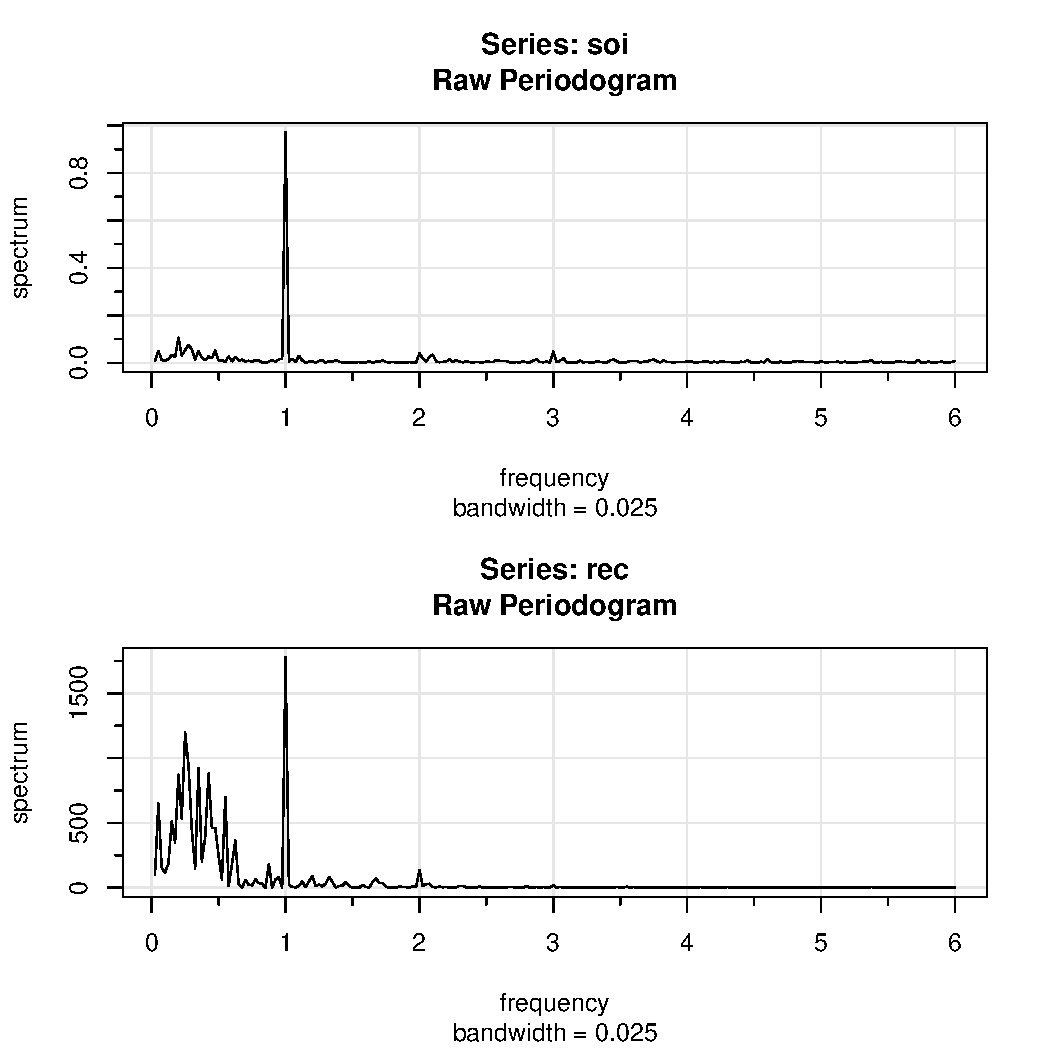
\includegraphics[width=110mm, height=75mm]{periodogram.pdf}

\end{frame}

\begin{frame}
\frametitle{Observations from Raw Periodograms}

From the raw periodograms:

\begin{itemize}
\item obvious peak at $\omega = 1/12$ for yearly cycle.
\item some peaks at around $\omega = 1/48$ for El Nino cycle. The wide band of activity suggests that this cycle is not very regular.
\end{itemize}

\end{frame}

\begin{frame}
\frametitle{Estimated Power and CIs from Raw Periodograms}

The estimates of the power spectra and the confidence intervals using the raw periodogram are listed below.

\begin{center}
\begin{tabular}{ccccc}
\hline \\
Series & $\omega$ & Estimated Power & Lower & Upper \\
\hline \\
SOI & $\frac{1}{48}$ & 0.0537 & 0.0146 & 2.1222 \\
    & $\frac{1}{12}$ & 0.9722 & 0.2636 & 38.4011 \\
    \hline\\
Recruit $(\times 10^3)$ & $\frac{1}{48}$ & 1.1974 & 0.3245 & 47.2935 \\
                        & $\frac{1}{12}$ & 1.7777 & 0.4819 & 70.2172 \\
\hline
\end{tabular}
\end{center}

\end{frame}

\begin{frame}
\frametitle{Apply Smoothing}

The periodogram might need smoothing to determine a predominant overall trend for El Nino. Applying $L=9$ seems to work well. The resulting bandwidth is $9/480 = 0.01875$. This means that with $L=9$, we are assuming an approximately constant spectrum over $0.01875/0.5 = 0.0375$ of the entire frequency interval $[0, 1/2]$.

\end{frame}

\begin{frame}
\frametitle{Smoothed Periodograms}

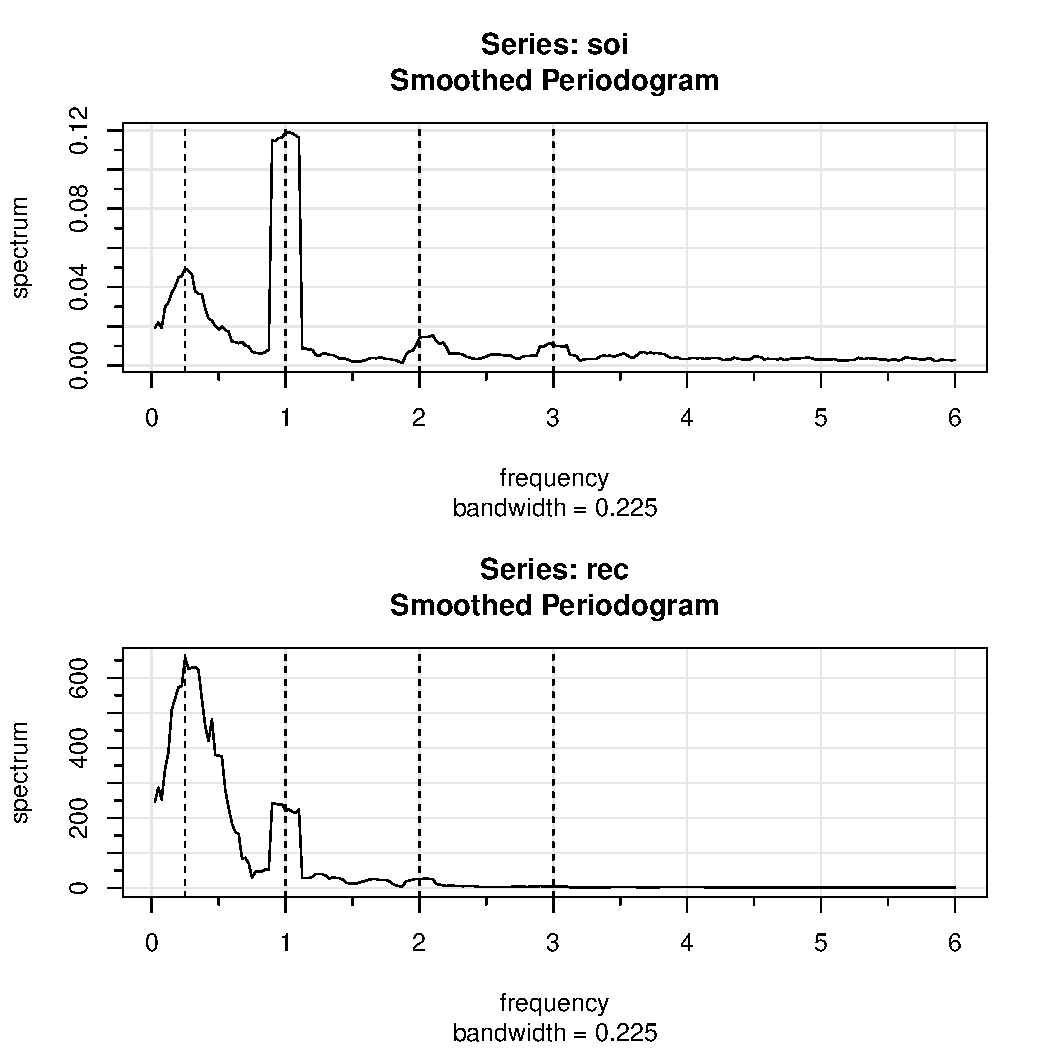
\includegraphics[width=110mm, height=75mm]{smoothed.pdf}

\end{frame}

\begin{frame}
\frametitle{Observations from Smoothed Periodograms}

From the smoothed periodograms:

\begin{itemize}
\item compromise with the noisy, unsmoothed version. Smoothing loses some of the peaks.
\item sharp peaks at $\omega=1/12$ now flattened to include nearby frequencies.
\item smaller flat peaks at multiples of $\omega=1/12$ appear.
\end{itemize}

\end{frame}

\begin{frame}
\frametitle{Estimated Power and CIs from Smoothed Periodograms}

The estimates of the power spectra and the confidence intervals using the symmetric average smoother with $L=9$ are listed below.

\begin{center}
\begin{tabular}{ccccc}
\hline \\
Series & $\omega$ & Estimated Power & Lower & Upper \\
\hline \\
SOI & $\frac{1}{48}$ & 0.0495 & 0.0279 & 0.1113\\
    & $\frac{1}{12}$ & 0.1191 & 0.0670 & 0.2677 \\
    \hline\\
Recruit $(\times 10^3)$ & $\frac{1}{48}$ & 0.6590 & 0.3710 & 1.4815 \\
                        & $\frac{1}{12}$ & 0.2194 & 0.1235 & 0.4932 \\
\hline
\end{tabular}
\end{center}

\end{frame}

\begin{frame}
\frametitle{Choice for Bandwidth}

From (\ref{eq:bandwidth}), the bandwidth is $B = L/n$. Here are some considerations as we decide the value of $L$ in the bandwidth:

\begin{itemize}

\item If $L$ is too large, our assumption that $f(\omega)$ is approximately constant within the frequency band may become more questionable. We may end up \textbf{smoothing out} valid peaks within a frequency band.

\item If $L$ is too small, the confidence intervals for $f(\omega)$ may become too wide, making it difficult to detect significance. 

\end{itemize}

What is normally done: vary the value of $L$ and examine the resulting periodograms to see if common observations can be made. 

\end{frame}


\section{Generalization of Smoothing}
\frame{\tableofcontents[currentsection]}

\begin{frame}
\frametitle{Generalization of Smoothing}

A generalization of smoothing for the periodogram is
\begin{eqnarray}\label{eq:1}
\widehat{f}(\omega)= \sum_{k=-m}^{m} h_k I(\omega_j + k/n)
\end{eqnarray}
where $h_{-k}=h_k>0$ and $ \sum_{k=-m}^{m}  h_k=1$. The asymptotic distribution of chi-squared continues to hold as $m/n \rightarrow 0$ which will give that $ \sum_{k=-m}^{m}  h_k^2 \rightarrow 0$.

\end{frame}




\begin{frame}
\frametitle{Generalization of Smoothing}

Under these conditions $E(\widehat{f}(\omega)) \rightarrow f(\omega)$.  This estimator also has the following asymptotic distribution

\begin{equation} \label{eq:asymp}
\frac{2 L_h  \widehat{f}(\omega)}{f(\omega)} \rightarrow \chi_{2 L_h}^2
\end{equation}
where $L_h = \left( \sum_{k=-m}^{m}  h_k^2 \right)^{-1}$.

\end{frame}

\begin{frame}
\frametitle{Generalization of Smoothing}

When we smooth a periodogram, we smooth across a frequency band. Recall that the periodogram is computed at the fundamental frequencies $\omega_j = j/n$ for $j=1, 2, \cdots, n/2$. When smoothing is applied to a periodogram, $\widehat{f}(\omega)$ is a \textbf{weighted average} of the periodogram values for frequencies in the range $\frac{j-m}{n}$ to $\frac{j+m}{n}$.

\end{frame}

\begin{frame}
\frametitle{Generalization of Smoothing}

Note that when we set $h_k = L^{-1}$ for all $k$, where $L=2m+1$, we obtain the symmetric moving average smoother we defined earlier in (\ref{eq:smooth}),

\begin{equation*}
\overline{f}(\omega)=\frac{1}{L} \sum_{k=-m}^{m} I(\omega_j + k/n).
\end{equation*}

\end{frame}

\begin{frame}
\frametitle{Bandwidth}

We earlier defined the bandwidth as $B = \frac{L}{n}$. The bandwidth is a measure of the width of the frequency intervals used for smoothing the periodogram. When \textbf{unequal weights} are used, this definition is modified to become

\begin{equation} \label{eq:band2}
B = \frac{L_h}{n} = \frac{1/ \sum_{k=-m}^{m} h_k^2}{n}.
\end{equation}

Equation (\ref{eq:band2}) holds for equal weights and is a generalization.

\end{frame}

\begin{frame}
\frametitle{CI for Smoothed Periodogram}

When using the smoothed periodogram as defined in (\ref{eq:1}), the approximate $(1-\alpha) \times 100\%$ confidence interval for the power spectrum at $\omega$ is

\begin{equation} \label{eq:CI2}
\frac{2 L_h   \widehat{f}(\omega)}{{\chi_{2L_h}^2(1-\alpha/2)}} \leq f(\omega) \leq \frac{2 L_h  \widehat{f}(\omega) }{{\chi_{2L_h}^2(\alpha/2)}} .
\end{equation}

If FFT and zero padding are used, then replace $2 L_h$ in (\ref{eq:CI2}) with $df = 2 L_h n / n^\prime$.

\end{frame}

\begin{frame}
\frametitle{Simultaneous CIs}

\begin{itemize}
\item In some situations, there is more than one frequency of interest, so we want to to make simultaneous inferences about the collection of frequencies we are interested in. 

\item To control the overall type I error rate, we work with the Bonferroni inequality $1 - K \alpha$ where $K$ denotes the number of frequencies we are interested in. 

\item Thus, to maintain $1 - \alpha$ confidence, the significance level for each frequency should be $\alpha/K$. 

\end{itemize}

\end{frame}

\begin{frame}
\frametitle{Simultaneous CIs}

The confidence interval (\ref{eq:CI2}) then becomes

\begin{equation} \label{eq:CI3}
\frac{2 L_h   \widehat{f}(\omega)}{{\chi_{2L_h}^2(1-\alpha/2K)}} \leq f(\omega) \leq \frac{2 L_h  \widehat{f}(\omega) }{{\chi_{2L_h}^2(\alpha/2K)}} .
\end{equation}

Going back to the worked example with the SOI and recruitment datasets, we constructed confidence intervals for the power spectrum at $\omega = 1/48$ and $1/12$. So $K=4$ if we want to have at least $95\%$ confidence that we do not make at least one type I error.

\end{frame}

%\begin{frame}
%\frametitle{Bandwidth}

%\begin{itemize}
%\item A bandwidth too great will oversmooth the periodogram and we may miss seeing important peaks.
%\item The bandwidth is predominantly controlled by the value $m$ or $L$, and whether we repeat the kernel (modified Daniell).
%\item It takes some experimentation to find a bandwidth that gives suitable smoothing.
%\item Note that the bandwidth reported in the periodogram in R is not calculated using formula (\ref{eq:band}).
%\end{itemize}

%\end{frame}


\section{(Modified) Daniell Kernel}
\frame{\tableofcontents[currentsection]}

\begin{frame}
\frametitle{Daniell Kernel}

Next, we explore some of the ways to generate the weights $h_k$, in R. A common choice for smoothing is to use the Daniell kernel. The Daniell kernel (initially) puts same
weights on neighbors.\\
\vspace{5mm}
\textbf{Question}: Does this sound familiar?

\end{frame}

\begin{frame}
\frametitle{Daniell Kernel}

For example, consider $m=1$ and
$L=2m+1=3$, the Daniell kernel has weights
$\{h_k\}=\{1/3,1/3,1/3\}.$ Applying this kernel to a sequence
 $\{u_t\}$ produces
$$
\hat{u}_t=\frac{1}{3} u_{t-1}+\frac{1}{3} u_{t}+\frac{1}{3} u_{t+1}.
$$

\end{frame}

\begin{frame}
\frametitle{Daniell Kernel}

We can apply the same kernel again to the $\hat{x}_t$ to obtain
\begin{eqnarray*}
\hat{\hat{u}}_t &=& \hspace{60mm} \\
                &=& \hspace{60mm}
\end{eqnarray*}



\end{frame}

\begin{frame}
\frametitle{Daniell Kernel}

Applying the Daniell kernel to obtain a smoothed periodogram as defined in (\ref{eq:1}), we
obtain

\begin{eqnarray*}
\widehat{f}(\omega) &=& \frac{1}{3} I(\omega_j - 1/n) + \frac{1}{3} I(\omega_j ) + \frac{1}{3} I(\omega_j + 1/n).
\end{eqnarray*}


\end{frame}


\begin{frame}
\frametitle{Daniell Kernel}

If we use the Daniell kernel twice, we obtain
\begin{eqnarray*}
\widehat{f}(\omega) &=& \frac{1}{9} I(\omega_j - 2/n) + \frac{2}{9} I(\omega_j - 1/n) +\frac{3}{9} I(\omega_j ) \\
                    &+& \frac{2}{9} I(\omega_j + 1/n) +\frac{1}{9} I(\omega_j + 2/n).
\end{eqnarray*}

A higher degree of smoothing is achieved by repeating the kernel.

\end{frame}

\begin{frame}[fragile]
\frametitle{Modified Daniell Kernel}

The modified Daniell kernel is such that the two endpoints in the averaging receive half the weight that the interior points do. For this example, the modified Daniell kernel puts one half on the center and one quarter on each. So, the sequence $\{u_t\}$ appears as follows:
$$
\hat{u}_t=\frac{1}{4} u_{t-1}+\frac{1}{2} u_{t}+\frac{1}{4} u_{t+1}.
$$

%Recall in \verb=spec.pgram()= function in R, we specify \verb?spans=3?.

\end{frame}

\begin{frame}[fragile]
\frametitle{Modified Daniell Kernel}

Applying the modified Daniell kernel again produces
\begin{eqnarray*}
\hat{\hat{u}}_t &=& \frac{1}{4} \hat{u}_{t-1}+\frac{1}{2}
\hat{u}_{t}+\frac{1}{4} \hat{u}_{t+1}\cr
&=&\frac{1}{16} u_{t-2}+\frac{4}{16} u_{t-1}+\frac{6}{16} u_{t}
+\frac{4}{16} u_{t+1}+\frac{1}{16} u_{t+2}.
\end{eqnarray*}

%In \verb=spec.pgram()= function in R, this kernel is specified by \verb?spans=c(3,3)?.

\end{frame}



\section{Worked Example}
\frame{\tableofcontents[currentsection]}

\begin{frame}
\frametitle{Worked Example}

We return to the SOI and recruit datasets. We use the modified Daniell kernel twice, with $m=3$ both times. This results in $L_h = 1/\sum_{k=-m}^{m} h_k^2 = 9.232$. The bandwidth now is $B = 9.232/480 = 0.019$. Compare these to $L=9$ and $B=0.01875$ from the earlier worked example, when we used the Daniell kernel.

\end{frame}

\begin{frame}
\frametitle{Raw Periodograms}

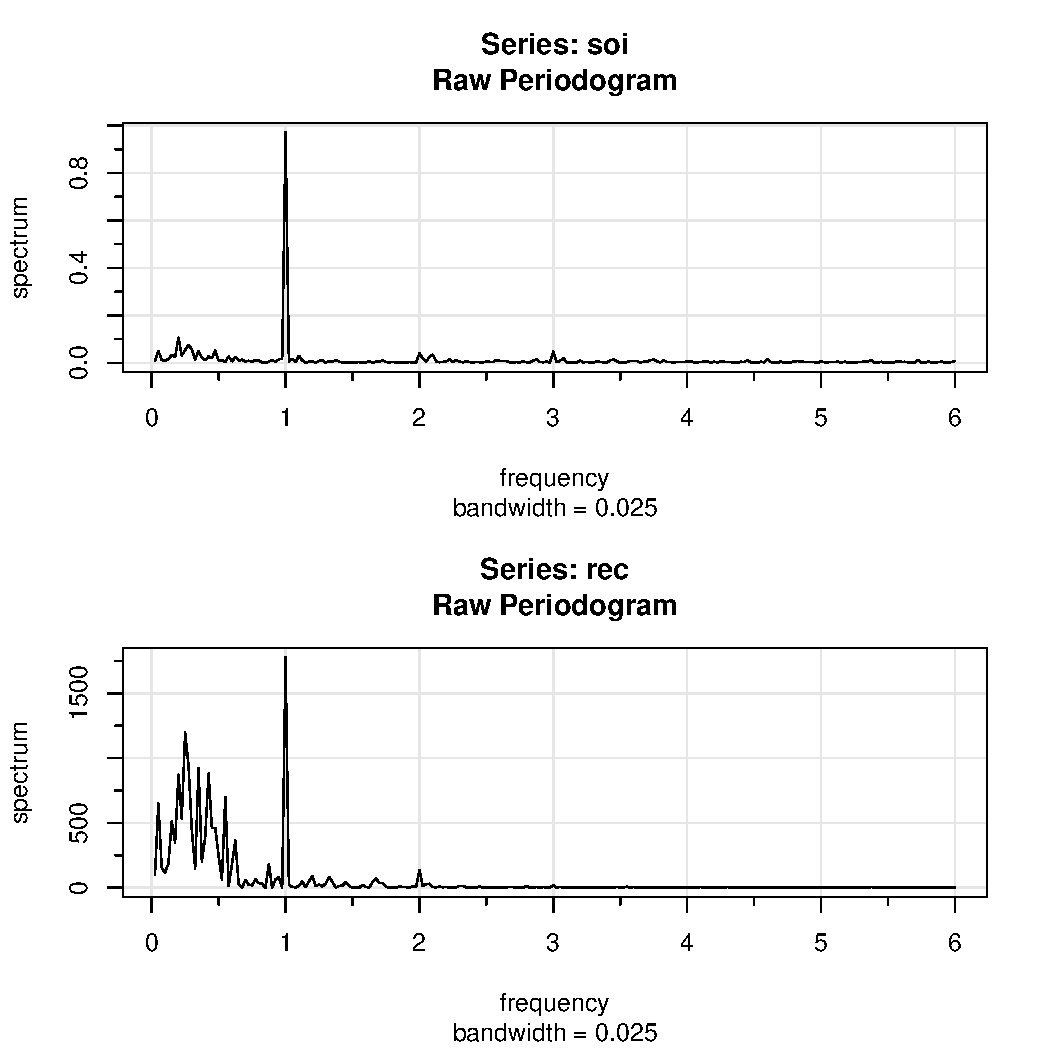
\includegraphics[width=110mm, height=75mm]{periodogram.pdf}

\end{frame}



\begin{frame}
\frametitle{Smoothed Periodograms with Modified Daniell Kernel}

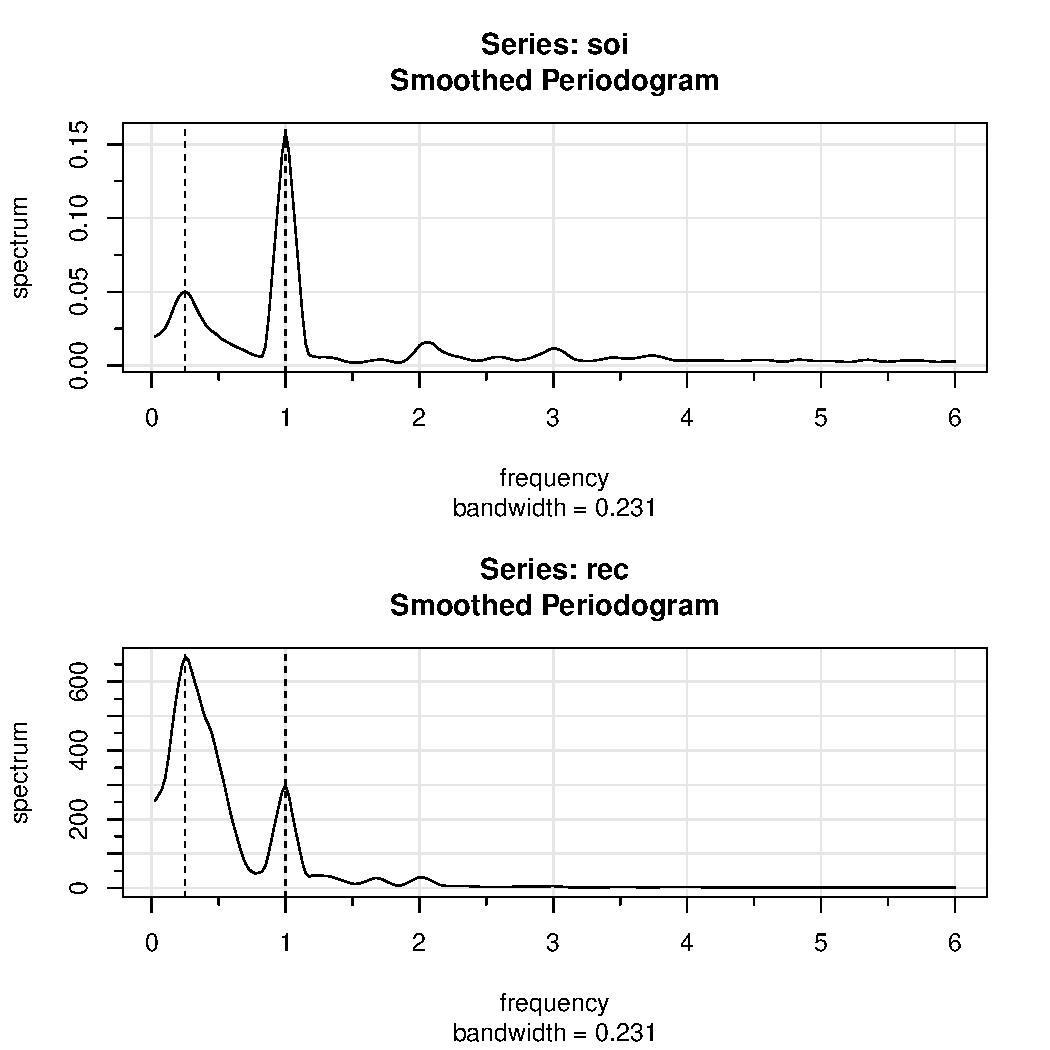
\includegraphics[width=110mm, height=75mm]{daniell.pdf}

\end{frame}

\begin{frame}
\frametitle{Estimated Power and CIs from Smoothed Periodograms}

The estimates of the power spectra and the confidence intervals using the modified Daniell kernel twice are listed below.

\begin{center}
\begin{tabular}{ccccc}
\hline \\
Series & $\omega$ & Estimated Power & Lower & Upper \\
\hline \\
SOI & $\frac{1}{48}$ & 0.0501 & 0.0284 & 0.1113\\
    & $\frac{1}{12}$ & 0.1582 & 0.0896 & 0.3513 \\
    \hline\\
Recruit $(\times 10^3)$ & $\frac{1}{48}$ & 0.6709 & 0.3801 & 1.4898 \\
                        & $\frac{1}{12}$ & 0.2981 & 0.1688 & 0.6619 \\
\hline
\end{tabular}
\end{center}

\end{frame}


\end{document} 